\documentclass[10pt]{article}
\usepackage[T1]{fontenc}

% Document Details
\newcommand{\CLASS}{AMATH 586}
\newcommand{\assigmentnum}{Assignment 3}

\usepackage[margin = 1.15in, top = 1.25in, bottom = 1.in]{geometry}

\usepackage{titling}
\setlength{\droptitle}{-6em}   % This is your set screw
\date{}
\renewcommand{\maketitle}{
	\clearpage
	\begingroup  
	\centering
	\LARGE \sffamily\textbf{\CLASS} \Large \assigmentnum\\[.8em]
	\large Tyler Chen\\[1em]
	\endgroup
	\thispagestyle{empty}
}
 % Title Styling
\usepackage{tocloft}
\renewcommand{\cfttoctitlefont}{\Large\sffamily\bfseries}
\renewcommand{\cftsecfont}{\normalfont\sffamily\bfseries}
\renewcommand{\cftsubsecfont}{\normalfont\sffamily}
\renewcommand{\cftsubsubsecfont}{\normalfont\sffamily}

\makeatletter
\let\oldl@section\l@section
\def\l@section#1#2{\oldl@section{#1}{\sffamily\bfseries#2}}

\let\oldl@subsection\l@subsection
\def\l@subsection#1#2{\oldl@subsection{#1}{\sffamily#2}}

\let\oldl@subsubsection\l@subsubsection
\def\l@subsubsection#1#2{\oldl@subsubsection{#1}{\sffamily#2}}
 % General Styling


\usepackage{enumitem}

% Figures
\usepackage{subcaption}

% TikZ and Graphics
\usepackage{tikz, pgfplots}
\pgfplotsset{compat=1.12}
\usetikzlibrary{patterns,arrows}
\usepgfplotslibrary{fillbetween}

\usepackage{pdfpages}
\usepackage{adjustbox}

\usepackage{lscape}
\usepackage{titling}
\usepackage[]{hyperref}


% Header Styling
\usepackage{fancyhdr}
\pagestyle{fancy}
\lhead{\sffamily \CLASS}
\rhead{\sffamily Chen \textbf{\thepage}}
\cfoot{}

% Paragraph Styling
\setlength{\columnsep}{1cm}
\setlength{\parindent}{0pt}
\setlength{\parskip}{5pt}
\renewcommand{\baselinestretch}{1}

% TOC Styling
\usepackage{tocloft}
\iffalse
\renewcommand{\cftsecleader}{\cftdotfill{\cftdotsep}}

\renewcommand\cftchapafterpnum{\vskip6pt}
\renewcommand\cftsecafterpnum{\vskip10pt}
\renewcommand\cftsubsecafterpnum{\vskip6pt}

% Adjust sectional unit title fonts in ToC
\renewcommand{\cftchapfont}{\sffamily}
\renewcommand{\cftsecfont}{\bfseries\sffamily}
\renewcommand{\cftsecnumwidth}{2em}
\renewcommand{\cftsubsecfont}{\sffamily}
\renewcommand{\cfttoctitlefont}{\hfill\bfseries\sffamily\MakeUppercase}
\renewcommand{\cftaftertoctitle}{\hfill}

\renewcommand{\cftchappagefont}{\sffamily}
\renewcommand{\cftsecpagefont}{\bfseries\sffamily}
\renewcommand{\cftsubsecpagefont}{\sffamily}
\fi
 % General Styling
% Code Display Setup
\usepackage{listings,lstautogobble}
\usepackage{lipsum}
\usepackage{courier}
\usepackage{catchfilebetweentags}

\lstset{
	basicstyle=\small\ttfamily,
	breaklines=true, 
	frame = single,
	rangeprefix=,
	rangesuffix=,
	includerangemarker=false,
	autogobble = true
}


\usepackage{algorithmicx}
\usepackage{algpseudocode}

\newcommand{\To}{\textbf{to}~}
\newcommand{\DownTo}{\textbf{downto}~}
\renewcommand{\algorithmicdo}{\hspace{-.2em}\textbf{:}}
 % Code Display Setup
% AMS MATH Styling
\usepackage{amsmath, amssymb}
\newcommand{\qed}{\hfill\(\square\)}

%\newtheorem*{lemma}{Lemma} 
%\newtheorem*{theorem}{Theorem}
%\newtheorem*{definition}{Definition}
%\newtheorem*{prop}{Proposition}
%\renewenvironment{proof}{{\bfseries Proof.}}{}


% mathcal
\newcommand{\cA}{\ensuremath{\mathcal{A}}}
\newcommand{\cB}{\ensuremath{\mathcal{B}}}
\newcommand{\cC}{\ensuremath{\mathcal{C}}}
\newcommand{\cD}{\ensuremath{\mathcal{D}}}
\newcommand{\cE}{\ensuremath{\mathcal{E}}}
\newcommand{\cF}{\ensuremath{\mathcal{F}}}
\newcommand{\cG}{\ensuremath{\mathcal{G}}}
\newcommand{\cH}{\ensuremath{\mathcal{H}}}
\newcommand{\cI}{\ensuremath{\mathcal{I}}}
\newcommand{\cJ}{\ensuremath{\mathcal{J}}}
\newcommand{\cK}{\ensuremath{\mathcal{K}}}
\newcommand{\cL}{\ensuremath{\mathcal{L}}}
\newcommand{\cM}{\ensuremath{\mathcal{M}}}
\newcommand{\cN}{\ensuremath{\mathcal{N}}}
\newcommand{\cO}{\ensuremath{\mathcal{O}}}
\newcommand{\cP}{\ensuremath{\mathcal{P}}}
\newcommand{\cQ}{\ensuremath{\mathcal{Q}}}
\newcommand{\cR}{\ensuremath{\mathcal{R}}}
\newcommand{\cS}{\ensuremath{\mathcal{S}}}
\newcommand{\cT}{\ensuremath{\mathcal{T}}}
\newcommand{\cU}{\ensuremath{\mathcal{U}}}
\newcommand{\cV}{\ensuremath{\mathcal{V}}}
\newcommand{\cW}{\ensuremath{\mathcal{W}}}
\newcommand{\cX}{\ensuremath{\mathcal{X}}}
\newcommand{\cY}{\ensuremath{\mathcal{Y}}}
\newcommand{\cZ}{\ensuremath{\mathcal{Z}}}

% mathbb
\usepackage{bbm}
\newcommand{\bOne}{\ensuremath{\mathbbm{1}}}

\newcommand{\bA}{\ensuremath{\mathbb{A}}}
\newcommand{\bB}{\ensuremath{\mathbb{B}}}
\newcommand{\bC}{\ensuremath{\mathbb{C}}}
\newcommand{\bD}{\ensuremath{\mathbb{D}}}
\newcommand{\bE}{\ensuremath{\mathbb{E}}}
\newcommand{\bF}{\ensuremath{\mathbb{F}}}
\newcommand{\bG}{\ensuremath{\mathbb{G}}}
\newcommand{\bH}{\ensuremath{\mathbb{H}}}
\newcommand{\bI}{\ensuremath{\mathbb{I}}}
\newcommand{\bJ}{\ensuremath{\mathbb{J}}}
\newcommand{\bK}{\ensuremath{\mathbb{K}}}
\newcommand{\bL}{\ensuremath{\mathbb{L}}}
\newcommand{\bM}{\ensuremath{\mathbb{M}}}
\newcommand{\bN}{\ensuremath{\mathbb{N}}}
\newcommand{\bO}{\ensuremath{\mathbb{O}}}
\newcommand{\bP}{\ensuremath{\mathbb{P}}}
\newcommand{\bQ}{\ensuremath{\mathbb{Q}}}
\newcommand{\bR}{\ensuremath{\mathbb{R}}}
\newcommand{\bS}{\ensuremath{\mathbb{S}}}
\newcommand{\bT}{\ensuremath{\mathbb{T}}}
\newcommand{\bU}{\ensuremath{\mathbb{U}}}
\newcommand{\bV}{\ensuremath{\mathbb{V}}}
\newcommand{\bW}{\ensuremath{\mathbb{W}}}
\newcommand{\bX}{\ensuremath{\mathbb{X}}}
\newcommand{\bY}{\ensuremath{\mathbb{Y}}}
\newcommand{\bZ}{\ensuremath{\mathbb{Z}}}

% alternative mathbb
\newcommand{\NN}{\ensuremath{\mathbb{N}}}
\newcommand{\RR}{\ensuremath{\mathbb{R}}}
\newcommand{\CC}{\ensuremath{\mathbb{C}}}
\newcommand{\ZZ}{\ensuremath{\mathbb{Z}}}
\newcommand{\EE}{\ensuremath{\mathbb{E}}}
\newcommand{\PP}{\ensuremath{\mathbb{P}}}
\newcommand{\VV}{\ensuremath{\mathbb{V}}}
\newcommand{\cov}{\ensuremath{\text{Co}\VV}}
% Math Commands

\newcommand{\st}{~\big|~}
\newcommand{\stt}{\text{ st. }}
\newcommand{\ift}{\text{ if }}
\newcommand{\thent}{\text{ then }}
\newcommand{\owt}{\text{ otherwise }}

\newcommand{\norm}[1]{\left\lVert#1\right\rVert}
\newcommand{\snorm}[1]{\lVert#1\rVert}
\newcommand{\ip}[1]{\ensuremath{\left\langle #1 \right\rangle}}
\newcommand{\pp}[3][]{\frac{\partial^{#1}#2}{\partial #3^{#1}}}
\newcommand{\dd}[3][]{\frac{\d^{#1}#2}{\d #3^{#1}}}
\renewcommand{\d}{\ensuremath{\mathrm{d}}}

\newcommand{\indep}{\rotatebox[origin=c]{90}{$\models$}}




 % Math shortcuts
% Problem
\usepackage{floatrow}

\newenvironment{problem}[1][]
{\pagebreak
\noindent\rule{\textwidth}{1pt}\vspace{0.25em}
{\sffamily \textbf{#1}}
\par
}
{\par\vspace{-0.5em}\noindent\rule{\textwidth}{1pt}}

\newenvironment{solution}[1][]
{{\sffamily \textbf{#1}}
\par
}
{}

 % Problem Environment

\newcommand{\note}[1]{\textcolor{red}{\textbf{Note:} #1}}

\hypersetup{
   colorlinks=true,       % false: boxed links; true: colored links
   linkcolor=violet,          % color of internal links (change box color with linkbordercolor)
   citecolor=green,        % color of links to bibliography
   filecolor=magenta,      % color of file links
   urlcolor=cyan           % color of external links
}


\begin{document}
\maketitle



\begin{problem}[Problem 1]
An ODE system, \({\bf u}'(t) = {\bf f} ( {\bf u} (t),t)\), \(t \geq 0\), is said to be {\em monotone} (with respect to the Euclidean inner product) if the real-valued function \({\bf f}\) satisfies
\[
\langle ( {\bf u}- {\bf v}) , {\bf f}({\bf u},t) - {\bf f}({\bf v},t) \rangle \leq 0
\]
for all \(t \geq 0\) and all vectors \({\bf u} , {\bf v} \in \mathbb{R}^d\).

\begin{enumerate}[label=(\alph*)]
\item Show that if \({\bf u}(t)\) and \({\bf v}(t)\) are two real solutions to a monotone ODE system with \({\bf u}(0) = {\bf u_0}\) and \({\bf v}(0) = {\bf v_0}\), then \(\| {\bf u}(t) - {\bf v}(t) \|\) decreases (weakly) monotonically for \(t \geq 0\). [Hint:  Look at $\frac{d}{dt} ( \| {\bf u} (t) - {\bf v} (t) \|^2 ) = \frac{d}{dt} \langle {\bf u}(t) - {\bf v}(t) , {\bf u}(t) - {\bf v} (t) \rangle$.]

\item Consider the linear ODE with variable coefficients
\[
{\bf u}' = A(t) {\bf u} ,~~~t \geq 0 ,
\]
where \(A\) is a real \(d\) by \(d\) matrix function of \(t\).  Prove that this ODE system is monotone if and only if all of the eigenvalues of the symmetric matrix \(B(t) = \frac{1}{2} [A(t) + A^T (t) ]\) are non-positive.

\item Suppose the backward Euler method is applied to the ODE system in part (b).  Let \(\{ {\bf U}^n \}_{n=0}^{n=N}\) be the sequence of vectors generated using initial value \({\bf U}^0\), and let \(\{ {\bf V}^n \}_{n=0}^{n=N}\)
be the sequence of vectors generated using initial value \({\bf V}^0 \) (and the same stepsize \(k\)). What conditions must \(k\) satisfy to ensure that \(\| {\bf U}^n - {\bf V}^n \|\) is a decreasing function of \(n \geq 0\)?
\end{enumerate}
\end{problem}

\begin{solution}[Solution]


\begin{enumerate}[label=(\alph*)]
    \item First observe that if \( g(t) = (g_1(t), \ldots, g_d(t)) \),
    \begin{align*}
        \dd{}{t} \ip{g(t),g(t)} = \dd{}{t} \left(g_1(t)^2 + \cdots + g_d(t)^2\right) = 2g_1(t)g_1'(t) + \cdots 2g_d(t)g_d'(t) = 2\ip{g(t),g'(t)}
    \end{align*}

    Suppose \( u(t) \) and \( v(t) \) are real solutions to a monotone ODE system. Then, since \( (u(t)-v(t))' = u'(t) -v'(t) = f(u,t) - f(v,t) \),
    \begin{align*}
    \dd{}{t} \norm{u(t)-v(t)}^2
    &= \dd{}{t} \ip{u(t)-v(t),u(t)-v(t)}
    = 2\ip{u(t)-v(t), f(u,t) - f(v,t)}
    \leq 0
    \end{align*}

    Therefore \( \norm{u(t)-v(t)}^2 \) is monotonically decreasing on \( [0,\infty) \). As \( \norm{u(t)-v(t)}\geq 0 \) on this interval, we also have that \( \norm{u(t)-v(t)} \) is monotonically decreasing on \( [0,\infty) \). \qed

    \item
    Observe, that if \( z,A(t) \) are real that \( A^H(t) = A^T(t) \) and \( \ip{z,A(t)z} \) is real. Therefore,
    \begin{align*}
        \ip{z,A(t)z} = \ip{A^H(t)z,z} = \overline{\ip{z,A^H(t)z}} = \ip{z,A^T(t)z}
    \end{align*}
    Using the above equality it is clear that,
    \begin{align*}
        \ip{z,B(t)z} =  \ip{z,\frac{1}{2}(A(t)+A^T(t))z} = \dfrac{1}{2}\ip{z,A(t)z} + \dfrac{1}{2}\ip{z,A^T(t)z} = \ip{z,A(t)z}
    \end{align*}

    Let \( v,w \in \RR^d \) and write \( z = v-w \). Since \( A(t) \) is linear,
    \begin{align*}
       \ip{u-v,A(t)(u-v)} = \ip{z,A(t)z} = z^TA(t)z
    \end{align*}

    Finally note that the eigenvalues of \( B(t) \) are all non-positive if and only if for all \( z \), \( \ip{z,B(t)z} \leq 0 \) (i.e. \( B(t) \) is negative semi-definite).

    This proves, the ODE system is monotone (\( \ip{u-v,A(t)(u-v)} = z^TB(t)z \leq 0 \) for all \( u,v \)) if and only all of the eigenvalues of \( B(t) \) are non-positive. \qed


    \item % see beginning of 7.4
    Backwards Euler gives,
    \begin{align*}
        (U^{n+1}-U^n)/k = A(t)U^{n+1} && \Longleftrightarrow &&
        U^{n+1} = (I-kA(t))^{-1} U^n = \left((I-kA(t))^{-1}\right)^{n+1}U^0 \\
        (V^{n+1}-V^n)/k = A(t)V^{n+1} && \Longleftrightarrow &&
        V^{n+1} = (I-kA(t))^{-1} V^n = \left((I-kA(t))^{-1}\right)^{n+1}V^0
    \end{align*}

    Therefore,
    \begin{align*}
        \norm{U^n - V^n} = \norm{\left((I-kA(t))^{-1} \right)^{n} (U^0-V^0)} \leq \norm{(I-kA(t))^{-1} }^{n} \norm{(U^0-V^0)}
    \end{align*}

    We should then pick \( k \) such that \( I-kA(t) \) is invertible and,
    \begin{align*}
        \norm{(I-kA(t))^{-1}} < 1
    \end{align*}

    Clearly a necessary condition for this is that \( |1-k\lambda_i| < 1 \) for \( i=1,\ldots, d \). (If \( A(t) \) is symmetric then this condition is also sufficient.)


\end{enumerate}

\end{solution}

\begin{problem}[Problem 2]
Consider the midpoint method \(U^{n+1} = U^{n-1} + 2k f( U^n )\) applied to the test problem \(u' = \lambda u\). The method is zero-stable and second order accurate, and hence convergent.  For \(\lambda < 0\) and any \(k > 0\),
however, the point \(z = k \lambda\) is {\em never} in the region of absolute stability of this method (see Example 7.7).  Thus the numerical solution will grow exponentially over time.  Yet the true solution \(u(t) = e^{\lambda t} u(0)\) decays exponentially over time.  How can numerical solutions that grow exponentially over time converge to something that decays exponentially over time?
\begin{enumerate}[label=(\alph*)]
\item To try and resolve this seeming paradox, let \(U^0 = \eta\), use forward Euler to generate \(U^1\), and then use the midpoint method for \(n=2,3, \ldots\).  Find an analytic expression for \(U^n\) by solving the linear difference equation.  What happens to this expression as \(k \rightarrow 0\)?
\item Devise some numerical experiments to illustrate the resolution of the paradox.
\end{enumerate}
\end{problem}

\begin{solution}[Solution]

\begin{enumerate}[label=(\alph*)]
    \item Using forward Euler we have,
    \begin{align*}
        U^1 = U^0 + k f(U^0) = U^0 + k\lambda U^0 = (1+k\lambda)\eta
    \end{align*}

    Using the midpoint method for \( n=1,2,\ldots \) we have difference equation,
    \begin{align*}
        U^{n+1} = U^{n-1} + 2kf(U^n) = U^{n-1} + 2k\lambda U^n
    \end{align*}

    Equivalently, for \( n=0,1,\ldots \)
    \begin{align*}
        U^{n+2} -2k\lambda U^{n} - U^{n} = 0, && U^0 = \eta, && U^1 = (1+k\lambda)\eta
    \end{align*}

    This has characteristic polynomial,
    \begin{align*}
        \chi(x) = x^2 - 2k\lambda x-1 = \left(x-k\lambda+\sqrt{1+k^2\lambda^2}\right)\left(x-k\lambda-\sqrt{1+k^2\lambda^2}\right)
    \end{align*}

    We therefore have general solution to the difference equations,
    \begin{align*}
        U^{n} = c_1 \left(k\lambda-\sqrt{1+k^2\lambda^2}\right)^n + c_2 \left(k\lambda+\sqrt{1+k^2\lambda^2}\right)^n
    \end{align*}

    Using the initial conditions we have,
    \begin{align*}
        \eta = c_1 + c_2, && (1+k\lambda)\eta = c_1 \left(k\lambda-\sqrt{1+k^2\lambda^2}\right) + c_2 \left(k\lambda+\sqrt{1+k^2\lambda^2}\right)
    \end{align*}

    This means,
    \begin{align*}
        c_1 = \frac{\eta  \left(\sqrt{k^2\lambda^2+1}-1\right)}{2 \sqrt{k^2\lambda^2+1}}, &&
        c_2 = \frac{\eta  \left(\sqrt{k^2\lambda^2+1}+1\right)}{2 \sqrt{k^2\lambda^2+1}}
    \end{align*}

    Therefore,
    \begin{align*}
        U^n = \left( \frac{\eta  \left(\sqrt{k^2\lambda^2+1}-1\right)}{2 \sqrt{k^2\lambda^2+1}} \right) \left(k\lambda-\sqrt{1+k^2\lambda^2}\right)^n + \left( \frac{\eta  \left(\sqrt{k^2\lambda^2+1}+1\right)}{2 \sqrt{k^2\lambda^2+1}}\right)  \left(  k\lambda+\sqrt{1+k^2\lambda^2}\right)^n
    \end{align*}

    Finally,
    \begin{align*}
        \lim_{k\to 0}U^n = \dfrac{\eta(1-1)}{2}(1) + \dfrac{\eta(1+1)}{2}(1) = \eta
    \end{align*}

    To explain the ``paradox'' consider the expression for \( U^n \) for \( k \) sufficiently small. In this limit we can take all \( \cO(k^2) \) terms to be zero. Then,
    \begin{align*}
        U^n = \dfrac{\eta(1-1)}{2})(k\lambda-1)^n + \dfrac{\eta(1+1)}{2} (1+k\lambda)^n = \eta (1+k\lambda)^n
    \end{align*}

    Now, with \( t = nk \) we have,
    \begin{align*}
    u(t) = \eta e^{t\lambda} = \eta e^{nk\lambda}= \eta \left( e^{k\lambda} \right)^n = \eta(1+k\lambda + \cO(k^2))^n
    \end{align*}

    These agree with one another for small enough \( k \).

    \item We take \( \eta = 1 \), \( \lambda = -10 \), and solve on \( [0,1] \) using the midpoint rule. We implement this in Python,
    \lstinputlisting[linerange=\#<start:mp>-\#<end:mp>]{hw3_2.py}

    Figure~\ref{midpoint} shows the results at various values of \( k \).

    \begin{figure}[H]\centering
        \foreach \n in {100,1000,3000,10000}{
            \begin{subfigure}{.48\textwidth}\centering
                \includegraphics[width=\textwidth]{img/mp_\n.pdf}
                \caption{ \( k=1/\n \)}
            \end{subfigure}
        }
    \caption{Midpoint method at various mesh sizes. Actual solution in grey.}
    \label{midpoint}
    \end{figure}

    Clearly the solution converges on our fixed, finite interval. However, it is also apparent that the solution will blow up if plotted on a larger interval (see analytic expression for \( U^n \) which diverges as \( n\to\infty \)). This is exactly in agreement with our definition for convergence.


\end{enumerate}


\end{solution}

\begin{problem}[Problem 3]
Use the boundary locus method described in Secs. 7.6.1-7.6.2 to plot the region of absolute stability for the TR-BDF2 method (8.6).  Observe that the method is A-stable and show that it is also L-stable.
\end{problem}

\begin{solution}[Solution]

Recall the TR-BDF2 method,
\begin{align*}
    U^{n+1} = \dfrac{1}{3}\left( 4U^*-U^n+kf(U^{n+1}) \right), &&
    U^* = U^n + \dfrac{k}{4}\left( f(U^n)+f(U^*) \right)
\end{align*}

Consider this method applied to the test equation \( u' = \lambda u \). Then,
\begin{align*}
    U^* = U^n + \dfrac{k}{4}(\lambda U^n + \lambda U^*) = U^n + \dfrac{k\lambda}{4}(U^n + U^*)
    && \Longleftrightarrow &&
    U^* = \left(\dfrac{1+k\lambda/4}{1-k\lambda/4}\right)U^n
\end{align*}

Therefore,
\begin{align*}
    U^{n+1} = \dfrac{1}{3} \left( 4\left(\dfrac{1+k\lambda/4}{1-k\lambda/4}\right)U^n - U^n + k\lambda U^{n+1}\right)
\end{align*}

Writing \( z = k\lambda \) we have,
\begin{align*}
    U^{n+1}\left( 1-\dfrac{z}{3} \right) = \dfrac{1}{3} \left( 4\left(\dfrac{1+z/4}{1-z/4}\right) - 1 \right) U^n
\end{align*}

Equivalently,
\begin{align*}
    U^{n+1} = R(z) U^n, && R(z) = \dfrac{12+5z}{12-7z+z^2}
\end{align*}

The region of stability is,
\begin{align*}
    \cS = \{z\in\CC : |R(z)| \leq 1\}
\end{align*}

To find the boundary of \( \cS \) we set \( R(z) = e^{i\theta} \),
\begin{align*}
    &12+5z = e^{i\theta} \left( 12-7z+z^2 \right) = 12e^{i\theta} - 7e^{i\theta}z + e^{i\theta}z^2
    \\ \Longleftrightarrow ~~~&
    e^{i\theta}z^2 - (7e^{i\theta}+5)z + 12e^{i\theta}-12 = 0
    \\ \Longleftrightarrow ~~~&
    z^2 - (7+5e^{-i\theta})z + 12(1-e^{-i\theta}) = 0
\end{align*}

This has solutions,
\begin{align*}
    z = \dfrac{(7+5e^{-i\theta})\pm \sqrt{(7+5e^{-i\theta})^2 - 4(12(1-e^{-i\theta}))}}{2}
\end{align*}

Figure~\ref{trbdf2} shows the contour plot of \( R(z) \) along with points of the form above evaluated at 30 values of \( \theta \) equally spaced from \( 0 \) to \( 2\pi \). Since \( R(z) \to 0 \) as \( z\to\infty \) we easily verify that \( \cS \) is the region on the outside of this boundary.
\begin{figure}[H]\centering
    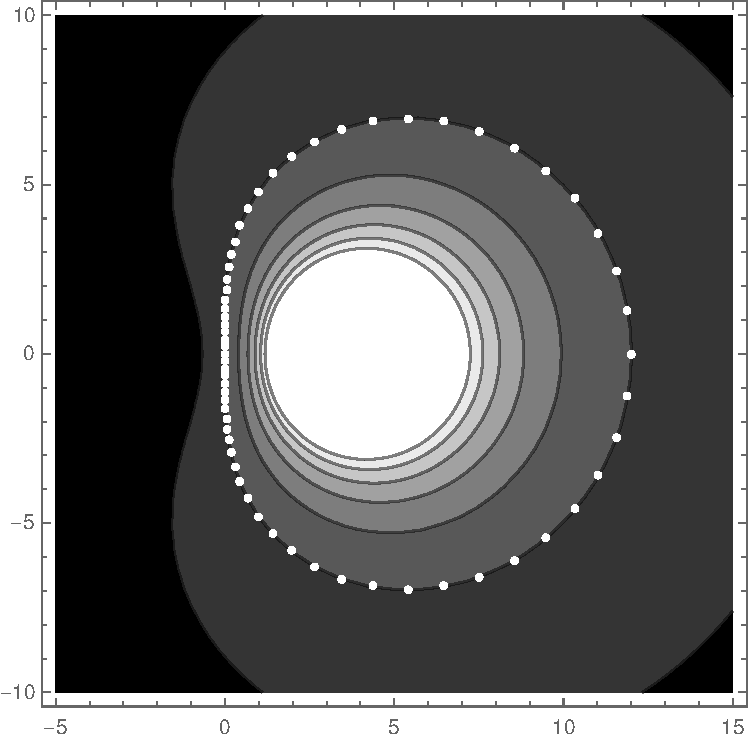
\includegraphics[width = 0.5\textwidth]{img/TRBDF2.pdf}
    \caption{Contour plot of \( R(z) \) and points evaluated on the boundary (white)}
    \label{trbdf2}
\end{figure}

Clearly the leftmost point of the boundary is \( z=0 \). Since \( R(0) = 1 \), the entire left half plane is contained in the region of stability. This means the method is \( A \)-stable.

Clearly \(  |R(z)| \to 0 \) as \( z\to\infty \) as the degree of the denominator of \( R(z) \) is larger than the degree of the numerator. This, along with \( A \)-stability  mean the method is also \( L \)-stable. \qed


\end{solution}

\begin{problem}[Problem 4]
Consider the A-stable trapezoidal method applied to the test problem \(u' = \lambda u\):
\[
U^{n+1} = U^n + \frac{k}{2} \lambda [ U^n + U^{n+1} ] .
\]
Of course, one can easily solve this linear equation for \(U^{n+1}\), but suppose we used {\em fixed point iteration} to solve for \(U^{n+1}\):  Taking \(w^{(0)}\) as an initial guess for \(U^{n+1}\), set
\[
w^{(j+1)} = U^n + \frac{k}{2} \lambda [ U^n + w^{(j)} ] ,~~~j=0, 1, \ldots .
\]
What conditions must \(k \lambda\) satisfy so that \(w^{(j)}\) will converge to \(U^{n+1}\)? [Note that if we use the trapezoidal rule but solve for \(U^{n+1}\) using fixed point iteration, we lose the benefits of A-stability!]
\end{problem}

\begin{solution}[Solution]


We write the iteration in the form,
\begin{align*}
    w^{(j+1)} = U^n + k\lambda (U^n + w^{(j)})/2
\end{align*}

Observe then that,
\begin{align*}
    \norm{w^{(j+1)} - U^{n+1}} &= \norm{(U^n + k\lambda (U^n + w^{(j)})/2) - (U^n + k\lambda (U^n + U^{n+1})/2) }
    = \dfrac{|k\lambda|}{2}\norm{ w^{(j)} - U^{n+1}}
\end{align*}

Therefore,
\begin{align*}
    \norm{w^{(j+1)} - U^{n+1}} = \left( \dfrac{|k\lambda|}{2} \right)^{j+1}\norm{w^{(0)}-U^{n+1}}
\end{align*}

This proves that fixed point iteration will converge if and only if \( k\lambda < 2 \). \qed


\end{solution}

\begin{problem}[Problem 5]
The following simple model describes the switching behavior for a muscle that controls a valve in the heart.  Let \(x(t)\) denote the position of the muscle at time \(t\) and let \(\alpha (t)\) denote the concentration at time \(t\) of a chemical stimulus. Suppose that the dynamics of \(x\) and \(\alpha\) are controlled by the system of differential equations
\begin{eqnarray*}
\frac{dx}{dt} & = & - \frac{x^3}{3} + x + \alpha \\
\frac{d \alpha}{dt} & = & - \epsilon x .
\end{eqnarray*}
Here \(\epsilon > 0\) is a parameter; its inverse estimates roughly the time that \(x\) spends near one of its rest positions.

\begin{enumerate}[label=(\alph*)]
\item Taking \(\epsilon = 1/100\), \(x(0) = 2\), and \(\alpha (0) = 2/3\), solve this system of differential equations using an explicit method of your choice.  Integrate out to, say, \(T = 400\), and turn in plots of \(x(t)\) and \(\alpha (t)\).  Explain why you chose the method that you used and approximately how accurate you think your computed solution is and why.
Comment on whether you seemed to need restrictions on the step size for stability or whether accuracy was the only consideration in choosing your step size.
\item
Solve the same problem using the backward Euler method and solving the nonlinear
equations at each step via Newton's method.  Write down the Jacobian matrix for the system and explain what initial guess you will use.  Were you able to use a larger time step using the backward Euler method than you were with the explicit method used in part (a)?
\end{enumerate}
\end{problem}

\begin{solution}[Solution]

\begin{enumerate}[label=(\alph*)]
    \item
        We implement forward Euler and the standard fourth order Runge-Kutta methods in Python:
        \lstinputlisting[linerange=\#<start:fw>-\#<end:fw>]{hw3_5.py}
        \lstinputlisting[linerange=\#<start:RK>-\#<end:RK>]{hw3_5.py}

        We pick these methods since they are the standard benchmarks for explicit one step methods. Our solutions do not really seem very accurate until at least \( N=600 \) at this point they seem to resemble the actual solution.

    \item
        Write,
        \begin{align*}
            f\left(\left[\begin{array}{c}x\\ \alpha\end{array}\right]\right) = \left[\begin{array}{c} -x^3/3 + x + \alpha \\ -\epsilon x \end{array}\right]
        \end{align*}

        Backwards Euler updates \( U^{n+1} \) by solving,
        \begin{align*}
            ( U^{n+1} - U^n )/k = f(U^{n+1})
        \end{align*}



        The Jacobian of \( f:\RR^2 \to \RR^2 \) is,
        \begin{align*}
            J_f(u)
              = \left[\begin{array}{cc}
                -x^2 + 1 & 1 \\
                -\epsilon & 0
            \end{array}\right]
        \end{align*}

        We apply Newton's method to solve for \( U^{n+1} \). At each step we compute,
        \begin{align*}
            w^{(j+1)} = w^{(j)} - \Delta w^{(j)}, && (I-kJ_f(w^{(j)})) \Delta w^{(j)} = w^{(j)} -k f(w^{(j)}) - U^{n}
        \end{align*}

        We will take \( w^{(0)} = U^n + k f(U^n) \), the value forward Euler would pick for \( U^{n+1} \) given current value \( U^{n} \). We iterate until the difference is around machine precision, or until we have reached our maximum iteration count (in our tests 100).

        We implement this in Python:
        \lstinputlisting[linerange=\#<start:bw>-\#<end:bw>]{hw3_5.py}

        \begin{figure}[H]\centering
        \foreach \t in {fe,rk,be}{ \foreach \n in {300,350,600}{
        \begin{subfigure}{.3\textwidth}\centering
            \includegraphics[width=\textwidth]{img/\t_\n.pdf}
          \caption{ \t, \( N = \n \)}
        \end{subfigure}
        }}
        \caption{Numerical solutions of \( x(t) \) (solid), \( \alpha(t) \) (dashed) on time interval \( [0,400] \) with output of Python's {\tt solve\_ivp} (with tolerance of \( 10^{-10} \)) shown in grey}
        \label{p5}
        \end{figure}


        While fewer mesh points are required for a reasonable solution, unless we iterate Newton's method for a long time, the solution does not always converge. When we allow Newton's method to converge more fully we can take larger steps and still have convergence. Sample outputs are shown in Figure~\ref{p5}.


\end{enumerate}

\end{solution}
\end{document}
